\section{Introduction}

Composed image retrieval (CIR) is a challenging image retrieval task where the query involves both a reference image and a relative caption~\cite{liu2021,vo2019,baldrati2022}. It aims to retrieve the target image that encompasses the specified changes provided by the relative caption while otherwise preserving the visual similarity to the reference image. This dual-modal approach enables users to express subtle differences—such as adjusting colours, styles, or shapes—in a more precise and intuitive manner, thereby enhancing retrieval accuracy and allowing for more precise control in describing the target image.

In the fashion domain, fashion image retrieval (FIR) is particularly compelling. FIR leverages visual cues and natural language inputs to precisely identify fashion items from vast repositories, allowing users to refine queries with modifying text—such as uploading an image of a dress and specifying ``make it in a pastel blue tone.'' This multimodal integration supports a range of applications in e-commerce, personalized shopping, and beyond, enabling searches based on sketches, textures, or contextual cues for events like weddings or job interviews. As the modern fashion industry is worth billions, breakthroughs in computer vision are revolutionizing trend forecasting, virtual try-ons, and inventory management.

Despite recent advances, FIR still has several limitations for application to real-world visual searches. These limitations include outdated and limited datasets that do not capture the diversity and variability of fashion items in the real world, the limited number of manually annotated triplets resulting in insufficient positive examples for effective contrastive learning, and triplet ambiguity, which refers to the difficulty in distinguishing between multiple images that may be visually similar to a query. These issues hinder the full potential of contrastive learning and highlight the need for more robust retrieval methods.

To address these issues, we propose a comprehensive framework that includes a multi-modal large language model to generate high-quality triplets and a two-stage fine-tuning framework. This framework aims to overcome the current limitations and improve the effectiveness of fashion retrieval systems.

Our contributions include:
\begin{itemize}
    \item Implementing a multi-modal large language model to generate high-quality triplets for contrastive learning.
    \item Developing a two-stage fine-tuning framework to enhance retrieval performance.
    \item Leveraging pretrained vision-language models to generate and concatenate sentence-level prompts with the relative caption.
\end{itemize}

\begin{figure}[t]
    \centering
    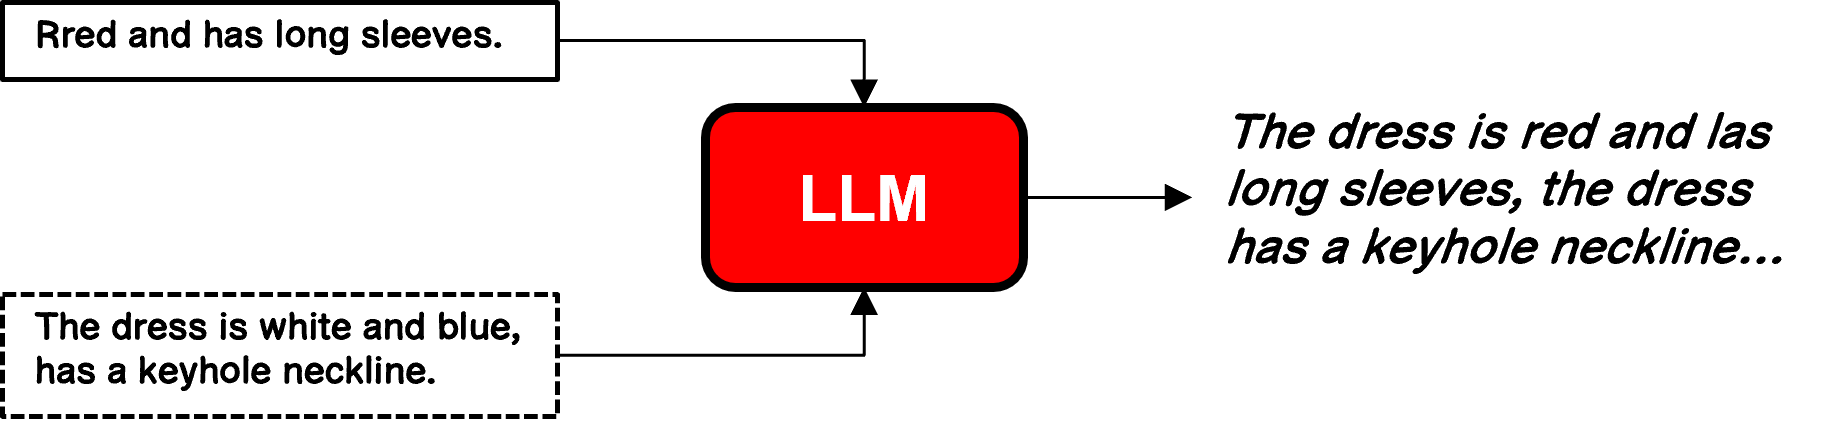
\includegraphics[width=\columnwidth]{figures/teaser.png}
    \caption{An example of using an LLM to enhance triplet quality.}
    \label{fig:teaser}
\end{figure}
